%%%%%%%%%%%%%%%%%%%%%%%%%%%%%%%%%%%%%%%%%%%%%%%%%%%%%%%%%%%%%%%%%%%%%%%%%%%%%%%%
% This chapter covers the design aspects, include design for data processing
% and the visual design
%
% - Add visual encoding nodes from MISC on google docs, probalby in the 3D
%   visualication subsection
% - Reference to WordNet
%%%%%%%%%%%%%%%%%%%%%%%%%%%%%%%%%%%%%%%%%%%%%%%%%%%%%%%%%%%%%%%%%%%%%%%%%%%%%%%%
\chapter{Design}


%%%%%%%%%%%%%%%%%%%%%%%%%%%%%%%%%%%%%%%%%%%%%%%%%%%%%%%%%%%%%%%%%%%%%%%%%%%%%%%%
\section{Data Processing}
In order to create our visualization, first we must be able to process and
extract semantics from our text collection. Our processing is broken down into 
two major stages, a preprocessing stage and an extraction/scoring stage. The 
preprocessing stage deals with normalizing the text and building a vocabulary 
of keywords that are used to represent the entities found in the document. 
The extraction/scoring stage scores each document the number of occurring keywords. 
Lastly, the final stage involves segmentation of \threed models into sub
subgroups such that each group can be semantically mapped against the keywords.

\subsection{Stage 1: Automatic Bootstrapping}
The foremost issue is to devise a method for extracting physical entities; a
document can contain multiple entities, but not all of which are related to the 
subject matter. On top of that, many entities can have implicit hierarchical 
relations, such as relation between component and its subcomponents. This 
relation is important because it enables logical groupings of entities.

Our entity extraction process leverages the WordNet database, a lexical English
database that stores nouns, verbs, adjectives and their relations among each
other \cite{WORDNET}. In order to get a comprehensive list of physical entities, we use the meronym 
relation in WordNet. A meronym describes a ``part-of'' relationship between two 
nouns, for example, a brake is a part of a wheel, and a wheel is a part of the 
automotive vehicle. All together, the meroynomy relationship forms a hierarchical 
structure where the most general part forms the root node, while the most specific 
parts form the leaf nodes. We use two common words pertaining to cars to bootstrap 
the hierarchy : ``car'' and ``vehicle''. From this we have two tree structures
rooted at ``car'' and ``vehicle'' respectively, we then merge the two
hierarchies, assuming that ``car'' and ``vehicle'' are equivalent. 

While this process extracts a fair amount of physical entities, it is not
representative of the entities being mentioned in the documents. The primary 
reason for this is due to the use of synonyms in the documents, where the object 
in question is using an alternative name. To alleviate some of these confusion, 
we additionally extract the synset relations from WordNet. A synset is a set of 
words are denoted to be semantically equivalent to each other, for example 
``limo'' and ``limousine'' are within the same synset.

The addition of synsets into the vocabulary gave us a comprehensive number of
keywords, however it also created undesirable noises. Manual examination of dataset 
sample reveal that there are still disconnects between the dictionary vocabulary 
and real world vocabulary. The next section we will describe how we overcome these issues.

\subsection{Stage 1: Manual Processing}
As an additional step to create our keyword vocabulary, we perform two manual
steps:
\begin{itemize}
  \item Removal of nouns that are too generic from the vocabulary.
  \item Preprocess the documents and mine for any missing nouns.
\end{itemize}
The first step deals with the removal of keywords that are not considered to be
physical objects under typical usage, for example WordNet hierarchy of car contains 
``first'', ``second'', ``third'' and ``fourth'', which describes the first,
second, third and fourth gears respectively. Including these words will likely result in 
over-counting the number of occurrences of gears than we should. We also removed 
several acronyms that will likely cause ambiguities, for example ``ice'', which
is short for internal-combustion-engine, will cause issues if the document is about ice, 
the solid state of water. They are therefore removed from the hierarchy. In the 
event where a node removal breaks the hierarchical structure, we simply connect 
the node�s children to the node�s parent.

The second step deals with any possible missing keywords that are not in WordNet
meronyms. We attempted to detect these semi-automatically with natural language 
processing techniques. We first perform part-of-speech (POS) tagging on our document 
corpus. POS taggers look at the grammatical structures of text and break down 
sentences into lexical categories such as nouns, verbs and adjectives. We use the 
POS output and tie them back to the original text, extracting the nouns and 
compound-nouns. We perform this step for all the documents in the corpus and 
count the number of occurrences for the nouns and compound-nouns. We then manually 
exam the top occurring words and add them into the hierarchy where we believe 
would be appropriate.

\subsection{Stage 1: Limitations}
While we believe this extract process is quite plausible method for building the
vocabulary, we acknowledge that WordNet is not the definitive authority for our 
problem domain, nor would it be for any specific domain. The keywords vocabulary 
can be extended and further refined by consulting experts that works in the 
problem field.

\subsection{Stage 2: Tagging}
For the actual matching, we use an open source, off the shelf snowball stemmer
before any matching takes place. Stemming is a process of reducing the words to 
their root forms. Finding the root is important because it unifies the singular 
and plural forms, as well, it converges various forms without the need to add 
additional vocabulary to our keywords. For the purpose of string matching, we 
perform stemming on both documents and key word vocabularies.

For the document text, stemming is performed on all string tokens and not
limited to nouns. This has both positive and negative effects. In our dataset, 
there are many objects with both noun and verb forms, for example ``braking
problem'' can be correctly associated with the keyword ``brake'' with stemming. On the 
other hand this also introduced false positives, the word ``lock'', which refers
to the component, is falsely picked up when the text describe components
``locking up''.

\subsection{Stage 2: Scoring Scheme}
Once we have identified the entities in each document, we can compute each
entity�s importance score. We denote the importance score of a physical object 
as the number of times it is mentioned within the document corpus. We have two 
primary metrics: occurrence  and co-occurrence. Within our problem context, the 
occurrence scores denotes the components that are most prone to failure, while 
the co-occurrence suggest causal relationships among the objects.

Let G be a (possibly empty) set of objects that are in the keyword hierarchy and
c be a single object in the hierarchy. We define a scoring function S(c, G) to be 
the total number of documents that have at least a single mention of c and G. Thus 
when G is the empty set the score is the absolute occurrence score (every document 
contains an empty set). When G is non-empty the score reflects the co-occurrence 
strength among a set of components. For clarity we illustrate this with a few examples:
\begin{itemize}
  \item $S(engine, \{\})$: The absolute strength of ``engine'' component in all
  documents
  \item $S(engine, \{engine\}$): The strength of ``engine'' relative to
  ``engine'', thus the same as the above
  \item $S(engine, \{brake\})$: The number of times engine keyword is mentioned
  when brake keyword is mentioned as well. Thus, mathematically,  $S(brake,
  \{\}) \geq S(engine, \{brake\})$
\end{itemize}


Each document is only counted once per object, this was done to discourage
biases coming from longer documents where the objects are repetitively mentioned.

\subsection{Stage 2: Limitations}
For this prototype, we gave the same score weighting to each objects. This is a 
subjective measure because not all parts are created equal. For example: if window 
is mentioned 10 times and the engine mentioned a single time, does that mean we 
should pay more attention to the window ? An extension to this work would be to 
devise an appropriate weighting scheme for our problem domain.

Another limitation is the vocabulary set itself, while we are only storing nouns 
as keywords, it would be interesting to look at verbs as well. For example, 
``stalled'', ``stalling'' are typically associated with engine object. Adding
verbs into our dictionary would give more flexibility and accurate results.

\subsection{Stage 3: Model Segmentation}
We use geometric models that compose of triangular mesh groups, where each mesh 
group can be uniquely identified and semantically mapped to our keyword ontology. 
The segmentation is done manually, with consultation of car schematics when it 
was not clear where the parts located. Where the model is missing parts, 
we add placeholder geometries.

We have chosen to use a sedan model as the starting point of our visualization. 
This was chosen based on the fact that sedans are the most common class of 
vehicles and best represent the dataset. We acknowledge that different types of 
vehicles may have different spatial arrangement of their components, we hope to 
remedy this as more vehicle models are processed.


%%%%%%%%%%%%%%%%%%%%%%%%%%%%%%%%%%%%%%%%%%%%%%%%%%%%%%%%%%%%%%%%%%%%%%%%%%%%%%%%
\section{Visual Design}
The following sections discuss our user interface and design decisions. In
summary, our interface is composed of five major components as seen in <Figure of overview>:
\begin{itemize}
  \item \threed Visualization:  The central point of the visualization system is
  a stylized rendering of the physical entities in the text documents (In our scenario, 
  a \threed rendering of a vehicle and its components).  The rendering is
  created in a way to emphasize the most highly scored object components so they are immediately 
  apparently to the readers via preattentive perception. The model can be interactively 
  rotated and zoomed in or out to explore different viewing angles and levels of detail.

  \item Time Filter: The time block filter is placed at the top-left of the
  screen. It allows selection of individual time periods, or the selection of a 
  contiguous block of time periods. The filters are subdivided into year and month 
  filters and corresponds to the entry date of the document.

  \item Hierarchy Filter:Domain Filter: The domain filters are placed at the
  bottom portion of the display akin to a series of drop-down menus. These are 
  designed specifically for our dataset of automotive complaints. The domain filters 
  allow successive query refinement by organizational hierarchies of manufacturers, 
  going in the order of : Vehicle Manufacturer, Vehicle Make, Vehicle Model and Vehicle Year.

  \item Lens Widget: The lens widget is used for exploring and querying \threed 
  space. The lens allows people to compose visual queries by positioning the lens 
  over the \threed visualization. The lens identifies the objects contained
  within it and displays additional information about them around the lens� circumference.

  \item Heatmap Widget: The heapmap show detailed information of each entity
  with respect to the selected time. The heatmap allows viewers to see trends
  and find outliers.

  \item Document Widget: The document widget displays the source text documents.
  The panel displays documents relating to the current selected objects and 
  highlights all component keywords.
\end{itemize}
In the following subsections we will describe each visualization components in
more detail, the trade offs and choices we made and our justifications.


\subsection{3D Visualization}
Data comes in many different dimensions, include those with spatial attributes
and those with abstract attributes. Our innovation is to show these spatial 
vocabulary as they would exist in the physical world, while using the abstract 
attributes as rendering parameters. For tasks related to word frequencies and 
other scores, we hypothesize that people will be able to see, and communicate 
better than in raw text formats because they are working with a familiar form. 
Proximity-based clusters formed in the spatial dimension would also encourage 
exploration of these areas that may otherwise go undetected. In our visualization, 
we use \threed models comprised of segmented sub-mesh groups that link to our
part-of relation hierarchy of component keywords.

In order to enhance the message carrying capacity of the visualization, we
considered several NPR techniques to encode the score onto each component objects. 
The encoding scheme should be clear and distinguishable by visual examination 
(Requirement R1), while maintaining the real world aspects. Our effects include 
varying stroke, halo/glow, colour variations, transparency effects and lighting 
effects. We chose colour mappings as our primary visual encoding, and use other 
effects as special effects and interactive highlights.

Designing a colour scheme for the encoding of the virtual component objects
presented several design trade-offs. We colour each object by mapping its score 
to a linear diverging yellow-orange-red hue scale, which is further divided into 
six discrete scoring bins. We display these hues as an on-screen legend at the 
bottom-left of the screen. We recognize that blending different hues in \threed
space does not necessarily produce a result which preserves the original hues, and can 
potentially lead to distracting visual artifacts. Different hue preservation 
schemes exist\cite{Chuang2009} but were not implemented for this prototype due
to the added performance complexity (Hue adjustments are done at per pixel levels). 
Due to known issues with blending, we have tried to use a single hue grey scale 
with varying brightness, but we found that it was somewhat difficult to distinguish 
overlapping or contained objects. Subjectively, single-hue also looks less 
aesthetically pleasing. Thus we decided that using a multi-hue scheme was 
more appropriate, despite the potential blending artifacts.

A second design trade-off was whether to use lighting effects or not. Lighting
effects such as specular lighting can create distractions because it can create 
highlights in places of little or no significance. Without any realistic lighting 
effects, or even simulated lighting effects, the visible colour of the components 
exactly matches the colour assigned to the score (and as seen on the legend). 
However, without any sort of lighting, particularly some type of diffuse lighting, 
the \threed nature of the model, and the details of various components are not
sufficiently visible. Adjacent objects that share the same score appear to be glued together 
as a single component, adding boundary outlines helps but creates additional 
clutters. When lighting effects are enabled, the objects are easily distinguishable 
as lighting provides a clear silhouette. However, this type of lighting modifies 
the colour based on the incidence angle of the light rays, thus it no longer matches 
the assigned colour. Ultimately our design decision is that object recognition and 
familiarity is important to us (R1). Thus, by restricting the number of hues (6 buckets) 
and using soft white light, we contend that the lighting effects do not disturb 
the colour perception enough to obscure which hue-bin the component belongs to. 
We made the design decision that the benefits of enabling lighting to visually 
resolve the components outweighed the negative effect of shifting colours away 
from those displayed in the onscreen legend.

In our design, we want to make all important objects visible (See requirement
R1), these includes objects partially or fully occluded by another object, and 
objects that are contained within others. The first case can be partially alleviated 
by changing the viewing distance and viewing perspective, whereas in the second case 
no amount of viewing adjustment will solve the occlusion issue. To address this 
problem, we double-encoded the importance score as both the colour and transparency 
values. The transparency value of each object is proportional to the object�s score, 
such that the higher scored objects appear more opaque, while the lower scored 
components appear more transparent. The maximum and minimum transparency values 
are capped at both ends such that no objects are completely opaque or completely 
transparent. One caveat of rendering translucent geometries in \threed space is
that ordering of geometries becomes important for blending to work correctly, 
out-of-sequence geometries appear to lose their depth cues when blended together. 
We will discuss this effect, and solutions in further detail in the 
implementation section. 

When the object�s score is zero, this indicates that there are no references of
the object in the documents that match the selected criteria. In this instance, 
we want to denote that this object is not important, while at the same time allowing 
the object to give some to the remaining components. Thus, rather than using colour 
and transparency as our encoding scheme, we extract edge geometries and render 
them in a faint, ghostly outline. We use a just-noticeable colour in order to 
provide context without distractions \cite{BAR2007a}. It is important to note
that zero objects are purely graphical artifacts and they do not partake in any 
user initiated interactions.

Since we are dealing with \threed geometry, it can be tempting to apply other
types of techniques. For example we attempted to encode the importance and other 
numerical semantics into the geometrical distortion that can be applied directly 
onto a \threed mesh. In practice, this does not work well for visual evaluation:
in general, objects are of different shapes and sizes, applying a small distortion 
is not entirely obvious while a large distortion can destroy the familiarity of 
the form. Yet another problem is that it is not possible to order or quantify by 
shape (Bertin), which makes the distortion a qualitative measure instead of a 
quantitative one. In addition, the ability to read quantitative value from a 
distortion field presumes that the viewer has a mental model of what the object 
looks like without any distortions, an assumption that we cannot make with our 
intended audiences.  However distortion remains an interesting possibility because 
we may use distortion to visually paint the action words, testing this will be 
part of our future work.


\subsection{Hierarchy Filter Widget}
The hierarchy widget is designed to model inclusive relationship, for our
problem domain, this relationship is represented as the organizational hierarchy. 
Our dataset contains 4 such fields: manufacturer, make, model and model year. 
For example: Civic (Make) belongs to Honda (Manufacturer). These filters are 
shown as a variant of the combo boxes which supports single selection, each item 
in the filter shows the name and the number of documents that belongs to it.

Rather than having the readers comparing items by reading the numbers in text
format, we double-encoded the number of document as a horizontal histogram in 
similar style as the scented widget approach \cite{Willett2007}. The
additional histogram makes it very clear any outlier items, and allows reader to make relative comparison 
among items. Toggling the widget will activate/deactivate the item list, which 
can be scrolled and selected, selected item is shown in bold font.

Each level of the hierarchy is shown in individual filters and its content is
dependent on the selection made on its parent. For example, the ``make''
selection widget will contain different makes if ``GM'' is the selected manufacturer than
it would for ``Chrysler''.  Non-top level hierarchy widgets remain hidden from view 
until it has selectable content, thus at the start, only the top level 
(manufacturer) filter widget is visible.

The hierarchical content is dependent on the currently selected time block. Our
application queries the document collection and reconstructs the hierarchy. Previous 
selected items are persisted if the items are available within the new selection 
criteria. In the case where the items do not exist, the widgets, and all their 
children widgets are hidden from view and we clear the corresponding selections.

\subsection{Time Filter Widget}
The time dimension is encoded as a histogram, with the height of each bar denoting 
the volume of unique complaints for that time period. There are several granularity 
options with our document collection: daily, weekly, monthly or yearly. From a 
preliminary analysis of the incoming volume of complaint documents, we found that 
daily and weekly granularity resulted in too much noises, there are insufficient
amount of data at that level to detect trends and other interesting patterns. Thus 
we selected to use month and year as our granularity levels. The widget consist of 
two sliders, the top slider represents time period in years, and the bottom slider 
represent time periods in months. Text labels at the top of each bar give the 
numerical representation of the volume of documents.

The widget allows people to select blocks of time, rather than a continuous time 
range. For example, selecting 2005 and 2006 on the year slider and March on the 
month slider, the querying time is exclusively March 2005 and March 2006. We believe 
that this feature is helpful for identifying repeating seasonal trends and for making 
comparison from season to season (\ie, All summer months versus all winter
month).
Thus the height of the month bar is tied to the accumulation of the volume of 
that month across all selected years. 

The current time selection can be changed by interacting with individual month or 
year bars (Clicking), or by dragging with the two markers at the base of each slider. 
Selections are highlighted, while non-selections are greyed out. Selection of an entire 
year (January to December) can be achieved using a double-clicking shortcut on the desired year.


\subsection{Lens Widget}
Using a metaphor of looking through a magnifying glass to reveal better detail
about a specific subject, we created an interactive widget to extract and show 
detailed information about entities in the text. This is in some sense a 
combination of filter plus detail-on-demand operations.

The lens widget operates in a hybrid \twod/\threed space, the lens itself exist
on a flat \twod surface, but it casts a cylindrical query volume into the
\threed visualization. Objects whose centroid are within the query volume are tagged, and have their 
detailed information displayed on the left/right sides of the lens as interactive 
information charts. A tagged object is identified with its chart by the use of 
line segments connecting the chart back to the component�s centroid location in 
screen space.

Each lens widget has its own rendering pipeline, as such, the focused area under
the lens can be rendered in a different styles, allows the objects to take up 
additional semantics and put further emphasis on the focus+context technique. 
For example, we can render the vehicle model with a flat opaque shading, while using 
transparency techniques for objects under the lens.

To build a rich, flexible query mechanism, the position of the lens and the
radius can be altered, thus creating different querying volume in different 
spatial locations. In addition, each lens widget use a depth parameter that acts 
as a cutting plane, all objects that comes before the cutting plane are excluded 
from the tagging process and are rendered as inactive objects. The depth parameter 
allows people to investigate occluded objects without resorting to changing their 
viewing perspectives.

Multiple lens widget are allowed to facilitate simultaneous exploration of
different areas, for example we can activate two lens, one examining the front
of the vehicle while the other examining the back of the vehicle. However we
have not defined any semantics for the lens to overlap, thus each lens should be
used individually.


\subsection{Heatmap Widget}
The information chart extruded from the lens widget is designed as a heatmap-like 
chart, it shows the volume of complaints registered against individual objects 
across time. Like our design for the time slider histograms, our intention is to 
allow people to compare specific periods of time across different years for a 
specific objects. The heatmap content corresponds to the currently selected time, 
it is also linked to other widgets as well as the \threed visualization, as
such, any query adjustments or selections will dynamically alter the heatmap.

Prior to our heatmap implementation, we have also considered using a simple 
scatter-plot, with time on the x-axis and the volume on the y-axis. While 
this solution is simpler to read and to detect long term trend it has two 
drawbacks: It does not allow easy comparison across different years, and it is 
not space efficient. Imagine the case where we have a 15 year period, it becomes 
difficult to compare year two versus year fourteen because they are too far apart, 
we also must allocate at least 180 pixels (One pixel minimum for each month) 
which takes up a lot of space.

We arrange the time segments chronologically onto a \twod grid like a calendar,
the month are arranged left-to-right in ascending order, and the years arranged 
top-to-bottom in ascending order. The months are thus horizontally aligned can 
be compared with relative ease, with each cell corresponding to the monthly score 
of the object. For consistency, we colour the cells using the same colour scale 
as the \threed visualization. Hovering over individual cells will cause a
tooltip to appear, showing the precise numerical score for the month, the tooltip itself is 
rendered with a semi-transparent style to avoid occlusion. Hovering also creates 
a highlight on the cell border, as well the same cell on all visible heatmap widgets 
are highlighted as a brush+link effect, this supports comparison across different 
object components.

The widget label, from left-to-right, shows the component name, the current
importance score, and the score if nothing is selected (The maximum score it 
can have). Since each component can correspond to multiple names, we label the 
component with the first name which appears in our vocabulary.

We have considered two types of labeling layout for our lens widget: A
flush-left/flush-right layout that places the heatmaps on either left or right 
side of the lens, and a radial layout where each heatmap is placed around the 
lens� circumference. The radial layout is anchored at the centre of the lens, 
imaginary line segments extends from the centre through the projected centroids,
and a real line segments extends the imaginary line to the circumference. The 
result was eye-pleasing, but due to the nature of the lens being an exploratory 
tool which gets moved around the screen frequently, the layout is unstable and 
not suited for this particular usage case. For the flush-based layout, we first 
sort the object centroids by their Y-coordinates in screen space, then we place 
the heatmaps on left/right side based on the heuristics below. Since there is 
no reliance on the centre of the lens for placement, moving the lens widget does 
not cause drastic changes to the heatmap placement and thus produce a more stable 
looking layout. Lastly we horizontally align the charts so it is easier for people 
to compare values across different heatmaps.

In order to avoid occluding the \threed visualization, or to run off screen
space, we employ the following heuristics.
\begin{itemize}
  \item Heatmap placement should always be outside of the axis-aligned bounding
  box (AABB) in projected screen space of the \threed visualization, unless the
  AABB itself runs off the screen.
  \item If the heatmaps are off the screen space, perform contraction to move it
  back into screen space.
\end{itemize}

Because of limited screen space, we have made the decision to limit the number
of heatmap that can be displayed at any given time. Rather than showing all the 
heatmaps under the lens widget, which would inevitably create visual clutter or 
having the heatmaps running off the screen, we use a scrolling mechanism that 
allows people to scroll through the focused objects. We have a parameter N which 
controls the maximum amount of visible heatmaps. We have no recommendations to 
what N should be, as it is specific to the data being visualized (number of entities) 
and the screen resolution. 


\subsection{Document Widget}
The document widget is the final stage of our drill-down process by providing links 
to the raw text. Each document is divided into two sections, the header section 
shows each document�s queryable attributes and the content section shows the raw 
text descriptions. Text are rendered on top of a semi-transparent panel and highlights 
are applied to selected object and co-occurring objects. To differentiated selected 
entities and related entities, we highlight selected entities in blue and related 
entities in grey, this creates a sharp contrast against the rest of the document text, 
allow readers to pick out the entities easily. 

By default the document widget is hidden from view as to not occlude the 
\threed visualization. Once the widget is toggled into existence, it can be
moved around the screen to user preferred position. Scrolling on the document widget 
is enabled if the contents overflow the display area. Scrolling is done at a pixel 
base level, rather than document base level. Pixel based scrolling is smoother, and 
are not prone to sudden changes in the visual display which can distract the readers. 
The technique we used to achieve this is to utilize alternating font-textures, 
this will be described in more detail in implementation section.


%%%%%%%%%%%%%%%%%%%%%%%%%%%%%%%%%%%%%%%%%%%%%%%%%%%%%%%%%%%%%%%%%%%%%%%%%%%%%%%%
\section{Interaction}
Interaction with the \threed model and interactive widgets dynamically update
the visualization to reflect any changes. The change of visualization state is carried 
through an animated transition that interpolates the colours and histogram values. 
In this section we describe the high-level interactions and models that 
support common tasks.

\subsection{Object Selection and Query Construction}
The current query criteria determines the visibility of the \threed objects, as
well as their selectability. Query is constructed by combining together selected values 
from widget instances and the selection buffer, which holds the currently selected 
objects. The system detects any changes to the query criterion and triggers the 
visualization to reevaluate. 

Object selection can be done in two ways: clicking on the \threed objects
themselves, or clicking on their representative heatmaps. In the case where objects occlude 
each other, selection will return the object that is closest to viewing point. 
In order to select occluded objects, the \threed model can be rotated to reveal
hidden entities. Alternatively, we can use the lens� depth functionality to cull away 
occluding geometries, or directly clicking on the heatmap representations which 
are always available. 

Selection is toggle based, thus clicking on a selected object or heatmap will 
de-select that item. Clicking on an empty space will trigger a reset and de-select 
all items. Selected items are accentuated visually with a glowing blue halo, this 
also applies to corresponding heatmaps which will have their border highlighted. 

Selected objects are added to the selection buffer, which also act as a query filter. 
When selection buffer is not empty, object scores are calculated in relation to 
the objects in the buffer, thus forming co-occurrence relations. For example, if 
we selected the �engine� and �door� objects in the visualization, the rest of the 
objects are recalculated to see if they co-occurs with both �engine� and �door�. 
By this convention, the selected objects will always have the maximal score after 
normalization, and will be coloured with the deepest shade on our colouring scale.

\subsection{Spatial Interaction}
The lens widget allows people to demand and filter detailed information by means
of of a visual query, people move the lens to inspect what they perceive to be 
interesting areas on the visualization. For any spatial or parameter changes in 
the lens, or changes to the \threed model�s orientation, we update the lens�
effect to reflect these changes to spatial coordinates. Unlike conventional systems 
where filters are explicitly stated (therefore requiring the users to have some 
notions of what they are looking for), our spatial interaction allows people to 
freely roam the visualization without prior knowledge or any explicit goals. Thus, 
this type of exploration may lead to people to discover things that are unknown to 
them before. For example, imagine a case where a strange noise is coming from the 
front of the car, while we do not have a clear idea of what component is causing
the noise, it is possible to use the lens widget to examine the �front� of the 
car for similar incident, and use the result to bootstrap our research effort.

\subsection{Surface Based Interaction}
We intended to have our application running on a walk-up-and-use large displays,
thus we have build our prototype to take into account keyboard/mouse free interactions. 
We use the idea of �zones� to process touch point events. Each interactive element 
has an implicit zone that is calculated when a touch point is detected by the 
sensor. The zones are either bounding boxes, or polygonal shapes that are detected 
using native picking support. An overview of different zones are as follows:
\begin{itemize}
  \item Visualization Zone: An axis-aligned bounding box that bounds the central
  visualization
  \item Time Block Zone: Covers the year/month sliders as well as their markers
  \item Filter Zone: Covers the accessible hierarchy filters
  \item Lens Zone: Area covered by the lens circumference
  \item Text Zone: Covers the document widget
  \item Empty Zone: An empty zone is none of the above.
\end{itemize}

Each touch point is tied to a single zone, and remains so until the touch point 
is removed. Thus, if we put our finger down at zone-A, and then we drag the finger 
to zone-B, the touch point is still registered with zone-A. This creates a 
continuous interaction and avoid distracting the users by sudden transition of different zones.
We designed the following gestures as our fundamental building blocks
\begin{itemize}
  \item Tap Gesture: Tap and lift finger.
  \item Hold: Tap and hold for at least X milliseconds
  \item Drag: Tap followed by move
  \item Flick: Tap followed by rapid move, the primary difference between a
  flick and a drag gestures is that we expect the velocity to be much greater with the flick gesture.
\end{itemize}
Higher level gestures are built by compositing together lower level gestures
\begin{itemize}
  \item Spread/Pinch: Dragging two touch point away or closer to each other, the
  two touch points need to start off in the same zone.
  \item 2-Finger Drag: Two point drags in the same direction. Where the two
  touch points are in the same zone and are close to each other.
  \item Hover: Hold followed by drag.
  \item 2-Tap: Two tap gestures in the same zone. We additionally differentiate
  whether the taps are close or far apart and allow different types to take on different semantics.
\end{itemize}
Our interactions with the system can be summarized by the table below: <Table>


\subsection{Visual Feedback}
When using the keyboard, mouse and other hardware peripherals, actions are
rewarded with some type of haptic feedback, for example we know when a key on a 
keyboard is pressed of depressed. This behaviour allows people to be more keenly 
aware of their current state. This is not true with touch interfaces, with touch 
sensing technology, it is possible for touch points to become lost during a gesture, 
this is due to the users accidentally lifting their fingers. When this happens people 
can get confused because they may be not be aware that their touch points are lost 
since their fingers are still contacting the table, there are no feedback system 
to alert the actual touch point had disappeared. To accommodate the lack of haptics, 
we implemented a visual feedback system. Whenever a touch point is registered, 
we render a gradient circle at the XY coordinates, the radius of the circle is 
adjusted such that it is large enough to be seen and not hidden under the fingertip. 
The circle is updated real with with respect to updates to the touch point, and 
is removed when the touch point is deregistered. Further, we also keep track up 
to the last 10 most recent updates of any active touch points and render them as 
breadcrumb trails. The trail gives additional visual clues to the type of 
gestures being performed.



%%%%%%%%%%%%%%%%%%%%%%%%%%%%%%%%%%%%%%%%%%%%%%%%%%%%%%%%%%%%%%%%%%%%%%%%%%%%%%%%
\section{Viewing Modes}
A comprehensive analytic system requires a variety of ways to manipulate and
looking at data. In this section we describe our solutions for trend detection,
making comparisons and high level overview.

\subsection{Heatmap Perspective}
The heatmap�s data, in essence, is a time series data. There are multiple ways
we can view this time series to derive interesting patterns and trends. For this 
prototype we want to concentrate on comparability across different components.
We have provided the following heatmap perspectives:
\begin{itemize}
  \item Month-Max: A monthly perspective where the importance score of each
  month is divided by the maximum monthly importance score over all components
  in the selected time block.
  \item Component-Max: An object component perspective where the importance
  score of each month is divided by the maximum component score over the selected time.
  \item Global-Max: A global perspective where the month score is divided by the
  maximum score of all components over the selected time. 
\end{itemize}
Each of the perspectives above answers different questions and has its own
advantages and disadvantages. The month-max perspective allows us to compare 
component-to-component by month, but comparison against adjacent cells are 
meaningless because each cell use a different maxima. The component-max 
perspective is the opposite, it allows us to see trends with a single object 
component, but it does not allow comparison across components. Lastly, the 
global-max perspective is good at showing the outliers and supports both 
month-to-month and component-to-component comparisons, but it can be difficult to 
see any trends in the non-outlier data because they are pushed into the bottom 
bins on the colour scale. To put the different modes in better context, we list 
sample questions that can be answered with these different perspective views:
\begin{itemize}
  \item Month-Max: In month X, which vehicle component had the most complaints?
  \item Component-Max: Are there more braking problems in the summer months or
  the winter month?
  \item Global-Max: What are the most unreliable vehicle components?
\end{itemize}
The perspective mode is changed via the dropdown list located at the bottom of
the user interface.

\begin{figure}
 \centering  
 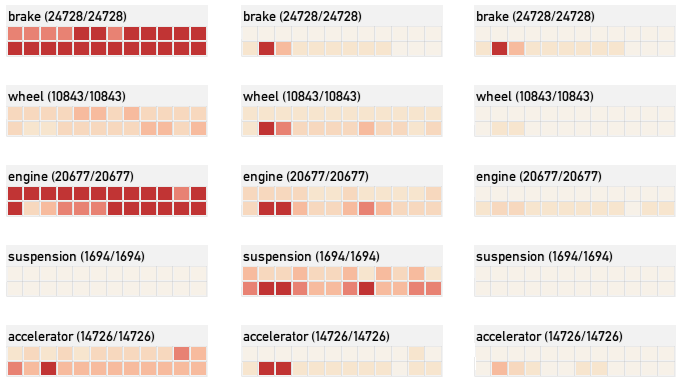
\includegraphics[width=\columnwidth]{heatmap.png}
 \caption{Showing the different heatmap perspectives. Left displays the monthly
 perspective, centre displays the component perspective, and right displays the
 global perspective}
 \label{figure:heatmap}
\end{figure}

\subsection{Comparison}
Comparison mode allows people to compare two different types of the same
physical product, for example: two different models of cars or two different 
manufacturers. Comparison are at the object level. Two different measures are 
used, the contribution sum and the contribution difference. The contribution sum 
is the aggregated score, it reflects the overall importance of the component with 
relations to other objects. The difference is the score of object one minus the 
score of object two, the sign, and the magnitude reflects which side has the 
stronger influence.

We encode the sum as object colour, based on the default colour scale. For the 
difference, we render the measure as an outline around the object. The sign of the 
difference is encoded as one of two diverging colours, one for positive and one 
for negative values. The magnitude of the difference is encoded as the transparency 
of the outline, larger magnitude have more distinct, solid outlines compared to 
smaller values. Thus, a highly problematic object from both side will have a 
strong presence overall but with a faint outline, while a lopsided but infrequent 
problem will have strong outline but barely visible interior colour.

The of the limitation in the current prototype is that we do not have any
normalization of comparative scores, thus it only makes sense comparing two 
different types of products with similar volumes.

\subsection{Aggregation}
By default, the system treats each object individually rather than object
groups. For example ``seatbelt'', ``backrest'' and ``seat'' are all scored
separately, even though they are logically under the group ``seat''. This
setting allows people to isolate and identify unique problems accurately. There
are times, however, when this level of information is unnecessarily detailed and
a higher level overview is desirable.

Aggregation mode mimics the type of high level rating system found on consumers
reivew websites. When aggregation mode is enabled, individual objects, and their
scores are aggregated up to the first level entities. In our specific case, the 
first level are the major sub-systems in a vehicle. The visualization responds
by making all child objects referencing the aggregated score of their parent
subsystem. 

Aggregation mode is enabled/disabled by a toggle switch located at the bottom
left of the user interface.

\begin{figure}
 \centering  
 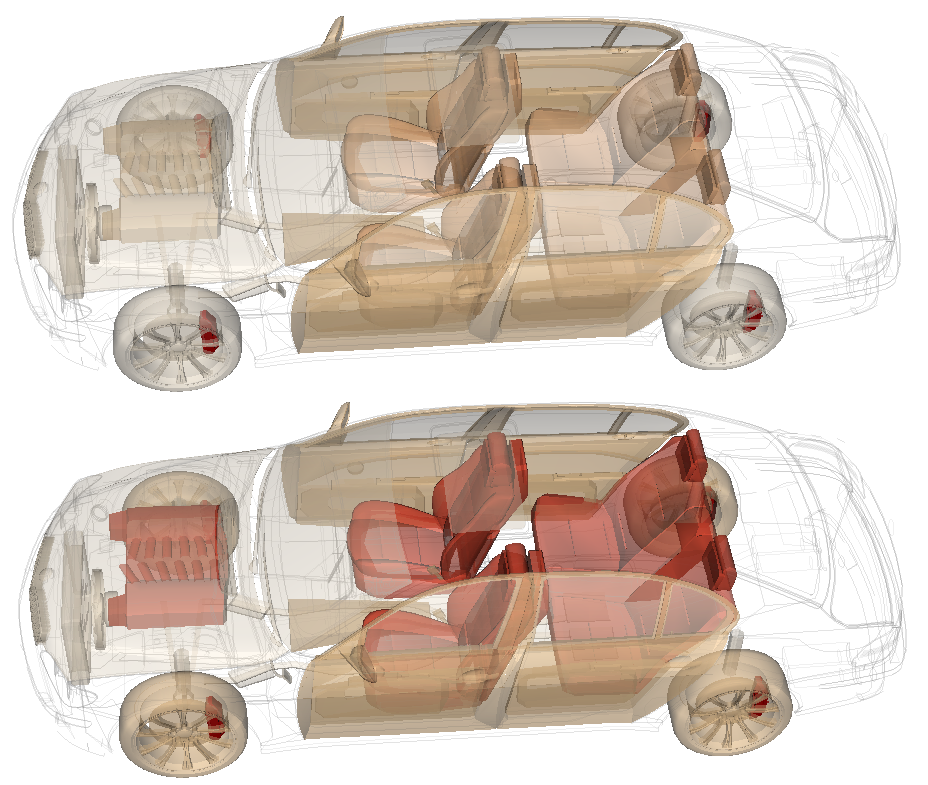
\includegraphics[width=\columnwidth]{aggregation.png}
 \caption{Top: Aggregation mode disabled. Bottom: Aggregation mode enabled,
 note that the seat and engine now appears more prominent in the visualization.}
 \label{figure:heatmap}
\end{figure}
